% Bao cao S^3 tieng Viet -- khuon ACL, dua tren acl_lualatex.tex (acl-org/acl-style-files)
% Bien dich bang XeLaTeX hoac LuaLaTeX (KHONG dung pdfLaTeX -- se loi font/dau tieng Viet).
% Tren Overleaf: Menu > Compiler > XeLaTeX (hoac LuaLaTeX), roi Recompile.
\documentclass[11pt]{article}

% "review" cho ban nop; doi thanh "final" khi nop ban cuoi (bo option nay).
\usepackage[review]{acl}
\usepackage{microtype}
\usepackage{graphicx}
\usepackage{booktabs}
\usepackage{amsmath}
\usepackage{amssymb}

% --- Font & tieng Viet: XeLaTeX/LuaLaTeX + babel, KHONG dung fontenc/inputenc kieu pdfLaTeX ---
\usepackage[vietnamese,english]{babel}   % vietnamese = ngon ngu phu (hyphenation); english = mac dinh cho tu khoa ACL
\babelfont{rm}{Noto Serif}   % font co chan, phu day du dau tieng Viet, co san tren Overleaf TeX Live
\babelfont{sf}{Noto Sans}
\babelfont{tt}{Noto Sans Mono}

\title{S\textsuperscript{3} cho Tiếng Việt: Tái lập, Đánh giá và Đề xuất Ứng dụng của Semantic Signal Separation}

% TODO: dien ten that + don vi cong tac truoc khi nop
\author{
  Tên Tác Giả 1 \\
  Trường/Khoa \\
  \texttt{email1@domain} \\\And
  Tên Tác Giả 2 \\
  Trường/Khoa \\
  \texttt{email2@domain}
}

\begin{document}
\maketitle

\begin{abstract}
% TODO: viet sau cung, ~150-200 tu, tom tat dong gop chinh.
Semantic Signal Separation (S\textsuperscript{3}) là một phương pháp mô hình
hoá chủ đề mới, coi mỗi chủ đề là một trục ngữ nghĩa độc lập được tách ra
bằng Independent Component Analysis (ICA) trên không gian embedding ngữ
cảnh. Báo cáo này tái lập S\textsuperscript{3} cho tiếng Việt, so sánh hai
encoder (CafeBERT và multilingual-E5), đề xuất một phương pháp đánh giá độ
chính xác bằng nhãn thật (điều paper gốc không thực hiện), và thử nghiệm
trên hai bộ dữ liệu tiếng Việt (ViSFD, VTSNLP). Nhóm cũng đề xuất và dựng
thử một ứng dụng định tuyến/giám sát dựa trên các trục ngữ nghĩa đã học.
\end{abstract}

\section{Giới thiệu}
\label{sec:intro}

Với sự bùng nổ dữ liệu văn bản tiếng Việt trên mạng xã hội, sàn thương mại
điện tử, và các nền tảng tin tức, nhu cầu tự động khám phá chủ đề/khía
cạnh ẩn trong khối lượng lớn văn bản -- mà không cần đọc thủ công từng tài
liệu -- ngày càng cấp thiết cho cả nghiên cứu học thuật lẫn ứng dụng doanh
nghiệp (giám sát phản hồi khách hàng, phân loại yêu cầu hỗ trợ...). Các mô
hình topic modeling cổ điển (LDA, LSA) và các hướng hiện đại hơn dựa trên
embedding ngữ cảnh (CTM, BERTopic, Top2Vec) đều đã được kiểm nghiệm rộng
rãi trên tiếng Anh, nhưng gần như chưa có công trình nào đánh giá một cách
có hệ thống trên tiếng Việt -- một ngôn ngữ đơn lập, viết cách âm tiết, đặt
ra thách thức riêng cho các bước tiền xử lý mà hầu hết mô hình mượn nguyên
từ tiếng Anh.

Semantic Signal Separation (S\textsuperscript{3}) \citep{kardos2025s3},
công bố tại ACL 2025, đề xuất một hướng tiếp cận khác biệt: thay vì coi
chủ đề là một cụm tài liệu hay một phân phối xác suất trên từ vựng, S³
định nghĩa chủ đề như một \emph{trục ngữ nghĩa} độc lập, tách ra từ không
gian embedding tài liệu bằng Independent Component Analysis (ICA). Cách
tiếp cận này không cần bước đếm từ (BoW/TF-IDF) để tìm chủ đề, chạy nhanh
hơn hẳn các baseline thần kinh, và mang lại một tính chất diễn giải độc
đáo mà các mô hình khác không có: \emph{định nghĩa âm} của chủ đề (từ khoá
cho biết chủ đề \emph{không phải} là gì). Tuy nhiên, mọi thực nghiệm trong
paper gốc đều chạy trên các kho ngữ liệu tiếng Anh, và paper cũng chủ động
không đánh giá độ chính xác của các trục ngữ nghĩa bằng nhãn thật cho bất
kỳ downstream task nào.

Báo cáo này đóng góp trên bốn khía cạnh, đúng theo yêu cầu đề tài. Thứ
nhất, nhóm \textbf{tái lập S\textsuperscript{3} cho tiếng Việt}
(Mục~\ref{sec:method}--\ref{sec:original-results} trình bày lại phương
pháp và kết quả gốc; Mục~\ref{sec:vn-experiments} là phần thực nghiệm của
nhóm), giải quyết một khác biệt kỹ thuật bắt buộc mà paper gốc không gặp
phải: tiếng Việt viết cách âm tiết, cần tách từ (word segmentation) trước
khi xây từ vựng, nếu không bước chiếu từ lên trục ngữ nghĩa
(Công thức~\ref{eq:projection}) sẽ vô nghĩa. Thứ hai, nhóm \textbf{so sánh
trực tiếp hai encoder} CafeBERT và multilingual-E5 (có thêm BGE-M3 làm đối
chứng) về cả tốc độ mã hoá lẫn độ chính xác trục ngữ nghĩa, trên hai bộ dữ
liệu tiếng Việt có nhãn thật độc lập: ViSFD (khía cạnh đánh giá điện
thoại, đa nhãn) và VTSNLP (domain nội dung, đơn nhãn). Thứ ba, nhóm đề
xuất và triển khai \textbf{một phương pháp đánh giá độ chính xác bằng
AUC} so trục ICA với nhãn thật -- điều paper gốc chủ động không làm -- trả
lời trực tiếp câu hỏi "một trục tìm được thuần tuý từ phương sai embedding
có thực sự trùng khớp với một khái niệm ngữ nghĩa có thật hay không?".
Thứ tư, nhóm dựng thử \textbf{hai ứng dụng chạy thật} dựa trên khả năng
suy luận tài liệu mới không cần huấn luyện lại của S\textsuperscript{3}
(Mục~\ref{sec:application}): một bảng điều khiển phát hiện bất thường và
một server định tuyến câu hỏi cho tổng đài ngân hàng.

Phần còn lại của báo cáo tổ chức như sau: Mục~\ref{sec:related-work} điểm
qua các hướng tiếp cận topic modeling hiện có và động lực dẫn tới
S\textsuperscript{3}; Mục~\ref{sec:method} trình bày chi tiết phương pháp
S\textsuperscript{3}; Mục~\ref{sec:original-results} tóm tắt kết quả thực
nghiệm của paper gốc; Mục~\ref{sec:vn-experiments} là phần thực nghiệm
trọng tâm của nhóm trên tiếng Việt; Mục~\ref{sec:application} trình bày
hai ứng dụng đề xuất; Mục~\ref{sec:conclusion} kết luận và nêu hạn chế.

\section{Công trình liên quan}
\label{sec:related-work}
% Nguon: report/section2_related_work.md (da duyet noi dung tieng Viet o do truoc,
% doan duoi day la ban da chuyen sang cu phap LaTeX).

Mô hình hoá chủ đề (topic modeling) là nhóm phương pháp thống kê không giám
sát nhằm khám phá các chủ đề ẩn trong một kho văn bản lớn mà không cần đọc
thủ công từng tài liệu, mỗi chủ đề thường được biểu diễn bằng một tập từ
khoá đại diện. Các phương pháp cổ điển như Latent Semantic Analysis (LSA)
\citep{deerwester1988lsa} và Latent Dirichlet Allocation (LDA)
\citep{blei2003lda} đều xây dựng trên biểu diễn Bag-of-Words (BoW) -- đếm
tần suất xuất hiện của từ, bỏ qua ngữ pháp và thứ tự từ. LSA nén ma trận
đếm từ xuống không gian có số chiều thấp hơn bằng phân tích giá trị kỳ dị
(SVD), trong khi LDA là một mô hình sinh xác suất, giả định mỗi tài liệu là
một phân phối Dirichlet trên các chủ đề rồi suy luận ngược bằng thống kê
Bayes. Cách tiếp cận dựa trên BoW gặp ba hạn chế cố hữu: (i) nhạy cảm với
các từ dừng (stop words) có tần suất cao nhưng không mang nội dung, khiến
chủ đề sinh ra thường lẫn nhiều từ vô nghĩa; (ii) đòi hỏi một khâu tiền xử
lý (loại bỏ từ dừng, chuẩn hoá từ...) không có chuẩn thống nhất, làm giảm
khả năng tái lập giữa các nghiên cứu; (iii) biểu diễn BoW rất thưa và có số
chiều cao, gây tốn kém tính toán và không nắm bắt được quan hệ ngữ nghĩa
giữa các từ đồng nghĩa hoặc đa nghĩa.

Sự xuất hiện của các mô hình biểu diễn ngữ cảnh dựa trên mạng nơ-ron sâu,
tiêu biểu là BERT \citep{devlin2019bert} và các biến thể tối ưu cho câu như
Sentence-BERT \citep{reimers2019sbert}, mở ra hướng đi mới: biểu diễn tài
liệu bằng vector đặc (dense embedding) mang thông tin ngữ cảnh, bền vững
hơn trước lỗi chính tả, và tận dụng được học chuyển giao (transfer learning)
từ mô hình đã huấn luyện trước trên kho ngữ liệu khổng lồ. Tuy nhiên, bản
thân embedding chỉ là một biểu diễn -- chưa phải là một mô hình chủ đề --
nên các phương pháp xây dựng trên nền tảng này chia thành hai nhánh chính.

\paragraph{Nhánh mạng nơ-ron (neural).} Contextualized Topic Models (CTM)
\citep{bianchi2021ctm} dùng một bộ tự mã hoá biến phân (VAE) nhận đầu vào là
embedding ngữ cảnh (có thể kết hợp thêm BoW) để tái tạo lại phân phối từ.
ECRTM \citep{wu2023ecrtm} bổ sung một cơ chế điều chuẩn phân cụm embedding
(embedding clustering regularization) để buộc các chủ đề tách biệt nhau rõ
hơn, còn FASTopic \citep{wu2024fastopic} mô hình hoá quan hệ tài liệu -- chủ
đề -- từ như một bài toán vận chuyển tối ưu (optimal transport). Điểm chung
của các mô hình này là vẫn cần một bộ giải mã hoặc hàm mất mát định nghĩa
trên không gian BoW, nên preprocessing nặng vẫn là một khâu khó tránh; đồng
thời quá trình huấn luyện lặp (nhiều epoch, tối ưu hoá hai giai đoạn) khiến
tốc độ chạy chậm và kết quả có thể không ổn định giữa các lần chạy.

\paragraph{Nhánh phân cụm (clustering).} Top2Vec \citep{angelov2020top2vec}
và BERTopic \citep{grootendorst2022bertopic} đi theo hướng hình học: dùng
UMAP \citep{mcinnes2018umap} để giảm chiều embedding xuống một không gian
vài chục chiều, sau đó dùng HDBSCAN \citep{campello2013hdbscan} để phân cụm
mật độ (density-based clustering) mà không cần định trước số cụm. Chủ đề
của mỗi cụm được suy ra hậu kỳ: Top2Vec dùng độ tương đồng cosine giữa
embedding từ và tâm cụm, còn BERTopic dùng một biến thể TF-IDF theo lớp
(class-based TF-IDF) -- tức là vẫn quay lại đếm từ ở bước cuối cùng.
Pipeline hai giai đoạn này (UMAP rồi HDBSCAN) có tổng cộng 5--6 siêu tham số
không có hướng dẫn lựa chọn rõ ràng, số cụm sinh ra không kiểm soát được
(có thể cần thêm bước gộp cụm), và một tài liệu bị phân sai cụm ở bước UMAP
sẽ không thể sửa được ở các bước sau.

\paragraph{Ba thách thức chung.} Nhìn xuyên suốt cả hai nhánh, các mô hình
chủ đề ngữ cảnh hiện có đối mặt với ba vấn đề: (1) nhạy cảm với lựa chọn
siêu tham số, khiến kết quả khó tái lập; (2) vẫn phụ thuộc vào một hình
thức đếm từ nào đó (BoW trong decoder của CTM, hay TF-IDF trong BERTopic),
nên chưa thực sự thoát khỏi hạn chế của cách tiếp cận cổ điển; (3) chưa có
bằng chứng rõ ràng cho thấy các mô hình này tận dụng được thông tin ngữ
cảnh thật sự, vì phần lớn được đánh giá trên dữ liệu đã qua tiền xử lý kỹ
lưỡng. Ba thách thức này chính là động lực trực tiếp dẫn tới Semantic
Signal Separation (S\textsuperscript{3}) \citep{kardos2025s3} -- phương
pháp mà nhóm tái lập và mở rộng cho tiếng Việt trong báo cáo này, được
trình bày ở Mục~\ref{sec:method}.

\section{Phương pháp: Semantic Signal Separation}
\label{sec:method}
% Nguon: main/content.md Act 3 (S10-S24).

\paragraph{Ý tưởng cốt lõi.} Khác với các mô hình được điểm qua ở
Mục~\ref{sec:related-work} -- vốn coi chủ đề là một phân phối xác suất trên
từ vựng (LDA) hoặc một cụm tài liệu (BERTopic, Top2Vec) -- S\textsuperscript{3}
\citep{kardos2025s3} định nghĩa lại chủ đề như một \emph{trục ngữ nghĩa}
(semantic axis): một hướng trong không gian embedding mà dọc theo đó, ý
nghĩa của văn bản biến thiên độc lập với các hướng khác. Định nghĩa này lấy
cảm hứng trực tiếp từ bài toán kinh điển trong xử lý tín hiệu gọi là
"cocktail party problem": khi nhiều nguồn âm thanh trộn lẫn vào nhau ở micro,
Independent Component Analysis (ICA) \citep{jutten1991ica,hyvarinen2000fastica}
có thể tách ngược lại các nguồn gốc độc lập chỉ từ tín hiệu trộn quan sát
được, không cần biết trước nguồn nào phát ra gì. S\textsuperscript{3} áp
dụng đúng nguyên lý đó cho embedding văn bản: coi mỗi embedding tài liệu là
một "bản trộn" của nhiều tín hiệu ngữ nghĩa độc lập (mỗi tín hiệu là một chủ
đề), rồi dùng ICA để tách các tín hiệu đó ra.

\paragraph{Quy trình sáu bước.} Gọi $X \in \mathbb{R}^{n \times d}$ là ma
trận embedding của $n$ tài liệu (mỗi hàng là vector $d$ chiều do một mô hình
encoder ngữ cảnh sinh ra, ví dụ Sentence-BERT). S\textsuperscript{3} tìm chủ
đề qua sáu bước:
\begin{enumerate}
    \item[(1)] \textbf{Mã hoá tài liệu}: dùng một encoder câu để biến $n$
    tài liệu thành ma trận $X$.
    \item[(2)] \textbf{Phân rã ICA}: áp dụng FastICA lên $X$ để thu được
    \begin{equation}
        X = A S,
        \label{eq:generative}
    \end{equation}
    trong đó $S \in \mathbb{R}^{n \times k}$ là ma trận $k$ thành phần độc
    lập (mỗi cột là một trục ngữ nghĩa -- một "chủ đề"), còn
    $A \in \mathbb{R}^{d \times k}$ là ma trận trộn (mixing matrix) biến các
    trục ngữ nghĩa trở lại không gian embedding gốc.
    \item[(3)] \textbf{Mã hoá từ vựng}: dùng cùng encoder ở bước (1) để mã
    hoá toàn bộ từ vựng của kho ngữ liệu thành ma trận
    $V \in \mathbb{R}^{m \times d}$ ($m$ là số từ).
    \item[(4)] \textbf{Ma trận giải trộn}: tính giả nghịch đảo
    Moore--Penrose của $A$,
    \begin{equation}
        C = A^{+},
        \label{eq:unmixing}
    \end{equation}
    đóng vai trò ánh xạ ngược từ không gian embedding về không gian trục
    ngữ nghĩa.
    \item[(5)] \textbf{Chiếu từ lên trục ngữ nghĩa}: dùng chính ma trận giải
    trộn $C$ để chiếu embedding từ vựng $V$ sang cùng không gian $k$ chiều
    với các trục chủ đề,
    \begin{equation}
        W = V C^{\top}, \quad W \in \mathbb{R}^{m \times k}.
        \label{eq:projection}
    \end{equation}
    \item[(6)] \textbf{Chấm điểm quan trọng của từ}: với mỗi trục $t$, sắp
    xếp các từ theo một trong ba công thức importance (trình bày dưới đây)
    tính từ cột $t$ của $W$, để chọn ra từ khoá đại diện cho chủ đề $t$.
\end{enumerate}
Vì bước (2) chỉ cần chạy FastICA -- một thuật toán hội tụ nhanh, không lặp
qua nhiều epoch như huấn luyện mạng nơ-ron -- toàn bộ pipeline có độ phức
tạp thấp hơn hẳn CTM hay ECRTM, và không cần bất kỳ bước đếm từ (BoW/TF-IDF)
nào để \emph{tìm} chủ đề: từ vựng chỉ được dùng ở bước (3)--(5) để
\emph{diễn giải} các trục đã tìm được. Nhóm dùng cấu hình FastICA đúng theo
Appendix C.1 của paper gốc (\texttt{algorithm="parallel"},
\texttt{whiten="unit-variance"}, \texttt{whiten\_solver="svd"}), triển khai
qua thư viện mã nguồn mở \texttt{turftopic} do chính nhóm tác giả
S\textsuperscript{3} công bố -- nhóm dùng lại thư viện này cho cả tái lập
lẫn thực nghiệm tiếng Việt ở Mục~\ref{sec:vn-experiments}.

\paragraph{Ba công thức chấm điểm quan trọng của từ.} Gọi $W_{jt}$ là toạ độ
của từ $j$ trên trục $t$ (phần tử hàng $j$, cột $t$ của $W$), và $\|W_j\|$
là độ dài vector embedding đã chiếu của từ $j$ trên toàn bộ $k$ trục (hình
chiếu của từ đó lên \emph{mọi} chủ đề, không riêng trục $t$). Hình~\ref{fig:word-importance}
minh hoạ trực giác hình học của ba công thức mà S\textsuperscript{3} đề
xuất:
\begin{align}
    \beta_{ax|t} &= W_{jt}, \label{eq:beta-axial}\\
    \beta_{ang|t} &= \frac{W_{jt}}{\|W_j\|}, \label{eq:beta-angular}\\
    \beta_{com|t} &= \frac{(W_{jt})^{3}}{\|W_j\|}. \label{eq:beta-combined}
\end{align}
Công thức \emph{axial} (\ref{eq:beta-axial}) chỉ lấy toạ độ thô trên trục
$t$, ưu tiên các từ có hình chiếu lớn nhất bất kể từ đó còn liên quan mạnh
đến các trục khác hay không. Công thức \emph{angular} (\ref{eq:beta-angular})
chuẩn hoá theo góc $\Theta$ giữa vector từ và trục $t$ (xem
Hình~\ref{fig:word-importance}), ưu tiên các từ mà gần như toàn bộ ý nghĩa
nằm dọc trục $t$, nhưng dễ bị nhiễu bởi các từ hiếm có $\|W_j\|$ rất nhỏ.
Công thức \emph{combined} (\ref{eq:beta-combined}) -- được paper gốc chọn
làm mặc định và cũng là công thức nhóm dùng xuyên suốt báo cáo này -- lấy
luỹ thừa bậc ba của $W_{jt}$ (giữ nguyên dấu vì số mũ lẻ, đồng thời khuếch
đại các giá trị lớn) rồi chuẩn hoá theo $\|W_j\|$ như công thức angular,
dung hoà giữa hai thái cực trên.

\begin{figure}[t]
    \centering
    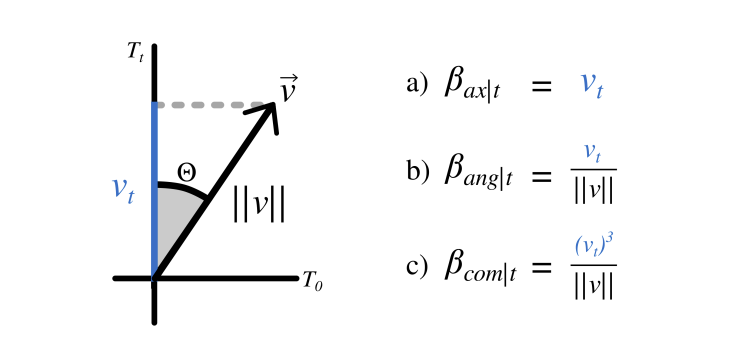
\includegraphics[width=\linewidth]{figures/figure3.png}
    \caption{Trực giác hình học của ba công thức chấm điểm quan trọng từ
    (axial, angular, combined). Tái hiện từ \citep{kardos2025s3}.}
    \label{fig:word-importance}
\end{figure}

\paragraph{Ý nghĩa âm: một chủ đề không chỉ được định nghĩa bởi những gì nó
là.} Vì $\beta$ có thể âm, mỗi trục ngữ nghĩa mang theo cả một tập từ có
trọng số dương lớn (\emph{định nghĩa dương} -- chủ đề \emph{là} gì) lẫn một
tập từ có trọng số âm lớn (\emph{định nghĩa âm} -- chủ đề \emph{không phải}
là gì, hay đối lập với nó). Đây là điểm khác biệt rõ rệt so với LDA hay
BERTopic, vốn chỉ liệt kê được từ khoá dương (xác suất hoặc tần suất luôn
không âm). Bảng~\ref{tab:arxiv-topics} minh hoạ điều này trên năm trục đầu
tiên mà S\textsuperscript{3} trích xuất từ một kho tóm tắt bài báo ArXiv về
Machine Learning: trục~3 chẳng hạn có định nghĩa dương xoay quanh đồ thị
(subgraph, graphsage) và định nghĩa âm xoay quanh tấn công đối kháng
(adversarial, security) -- hai chủ đề khác nhau nhưng cùng nằm trên một trục
lưỡng cực, cho thấy chúng có xu hướng \emph{loại trừ nhau} trong kho ngữ
liệu này.

\begin{table}[t]
    \centering
    \small
    \begin{tabular}{@{}c p{3.3cm} p{3.3cm}@{}}
        \toprule
         & \textbf{Từ trọng số dương} & \textbf{Từ trọng số âm} \\
        \midrule
        0 & clustering, histograms, clusterings, histogram, classifying &
        reinforcement, exploration, planning, tactics, reinforce \\
        1 & textual, pagerank, litigants, marginalizing, entailment &
        matlab, waveforms, microcontroller, accelerometers,
        microcontrollers \\
        2 & sparsestmax, denoiseing, denoising, minimizers, minimizes &
        automation, affective, chatbots, questionnaire, attitudes \\
        3 & rebmigraph, subgraph, subgraphs, graphsage, graph &
        adversarial, adversarially, adversarialization, adversary,
        security \\
        4 & clustering, estimations, algorithm, dbscan, estimation &
        cnn, deepmind, deeplabv3, convnet, deepseenet \\
        \bottomrule
    \end{tabular}
    \caption{Năm chủ đề đầu tiên trích xuất từ kho ArXiv ML Papers, mỗi chủ
    đề đi kèm định nghĩa dương và âm. Tái hiện từ \citep{kardos2025s3}.}
    \label{tab:arxiv-topics}
\end{table}

\paragraph{Concept Compass: trực quan hoá hai trục cùng lúc.} Vì mỗi từ và
mỗi tài liệu đều có toạ độ trên mọi trục, chọn hai trục bất kỳ làm hai trục
của một biểu đồ phân tán (scatter plot) cho phép quan sát trực tiếp cách các
khái niệm sắp xếp trong không gian ngữ nghĩa hai chiều đó -- tác giả gốc gọi
công cụ này là \emph{Concept Compass}. Hình~\ref{fig:concept-compass} là ví
dụ trên cùng kho ArXiv ML Papers, dùng trục 4 ("Deep Learning vs.\
Algorithms") làm trục tung và trục 1 ("Physical/Biological/Vision vs.\
Linguistic Problems") làm trục hoành: các từ liên quan đến thị giác máy
tính và robot học tụ ở góc trên-trái, các từ liên quan đến embedding và
ngôn ngữ tụ ở góc dưới-phải, trong khi các từ thống kê/thuật toán chung tụ
dọc trục tung phía trên -- một cấu trúc ngữ nghĩa mạch lạc mà không cần bất
kỳ nhãn giám sát nào.

\begin{figure*}[t]
    \centering
    
\includegraphics[width=0.75\linewidth]{figures/figure7.png}
    \caption{Concept Compass: các khái niệm được S\textsuperscript{3} sắp
    xếp theo hai trục ngữ nghĩa trên kho ArXiv ML Papers. Tái hiện từ
    \citep{kardos2025s3}.}
    \label{fig:concept-compass}
\end{figure*}

\paragraph{Suy luận cho tài liệu mới.} Một ưu điểm thực dụng của
S\textsuperscript{3} là suy luận toạ độ ngữ nghĩa cho một tài liệu chưa
từng thấy không đòi hỏi huấn luyện lại mô hình. Với một tài liệu mới được
mã hoá thành embedding $\hat{x} \in \mathbb{R}^{d}$ (hoặc một lô
$\hat{X} \in \mathbb{R}^{n' \times d}$), toạ độ trên $k$ trục ngữ nghĩa
được suy ra chỉ bằng một phép nhân ma trận với ma trận giải trộn $C$ đã
tính ở bước (4):
\begin{equation}
    \hat{S} = \hat{X} C^{\top}.
    \label{eq:inference}
\end{equation}
Vì Công thức~\ref{eq:inference} chỉ là một phép nhân ma trận không tốn kém,
S\textsuperscript{3} có thể suy luận theo thời gian thực cho luồng dữ liệu
mới -- tính chất mà nhóm khai thác trực tiếp cho đề xuất ứng dụng ở
Mục~\ref{sec:application}.

\section{Kết quả thực nghiệm gốc (tóm tắt)}
\label{sec:original-results}
% Nguon: main/content.md Act 4 (S25-S32).

\paragraph{Thiết lập thực nghiệm.} Paper gốc đánh giá S\textsuperscript{3}
trên năm kho ngữ liệu tiếng Anh -- ArXiv ML Papers, BBC News, 20
Newsgroups, StackExchange, Wiki Medical -- với 20 Newsgroups được chạy ở cả
hai biến thể văn bản thô (raw) và đã tiền xử lý (preprocessed) để riêng đo
ảnh hưởng của tiền xử lý, tổng cộng sáu bộ dữ liệu thí nghiệm. Bốn mô hình
encoder được so sánh, trải từ embedding tĩnh cổ điển đến ngữ cảnh hiện đại:
GloVe, all-MiniLM-L6-v2, all-mpnet-base-v2, và intfloat/e5-large-v2. Số
lượng trục/chủ đề được quét từ 10 đến 50. Để tránh p-hacking, nhóm tác giả
không tinh chỉnh siêu tham số cho bất kỳ mô hình nào và chỉ chạy một lần
duy nhất cho mỗi cấu hình -- nhóm chúng tôi tái dựng đúng thiết lập này
bằng gói \texttt{topic-benchmark} (mã nguồn mở do chính nhóm tác giả
S\textsuperscript{3} công bố) để có các hình trong mục này.

\paragraph{Cách đo chất lượng.} Hai tiêu chí chính được dùng: \emph{Diversity}
($d$) đo mức độ khác biệt giữa các chủ đề (tỷ lệ từ khoá không trùng lặp
giữa các topic), và \emph{Coherence} ($C$) đo mức độ mạch lạc nội tại của
từng chủ đề, được tính từ hai thành phần external/internal word-embedding
coherence rồi gộp bằng trung bình nhân $\bar{C}=\sqrt{C_{ex} \cdot C_{in}}$.
Một chỉ số tổng hợp thứ ba, \emph{Interpretability}~$=\sqrt{\bar{C} \cdot d}$,
cũng dùng trung bình nhân để phạt nặng mô hình lệch mạnh về một trong hai
mặt (đa dạng cao nhưng vô nghĩa, hoặc mạch lạc cao nhưng trùng lặp).

\paragraph{Tốc độ: kết quả nổi bật nhất.} Hình~\ref{fig:runtime} là bằng
chứng rõ nhất: trên toàn bộ 20 tổ hợp (5 kho $\times$ 4 encoder), thời gian
chạy của ba biến thể S\textsuperscript{3} (đường xanh dày, gần như trùng
nhau vì ba công thức word-importance chỉ khác nhau ở bước hậu xử lý, không
ảnh hưởng thời gian phân rã ICA) luôn nằm ở đáy biểu đồ trục tung logarit,
cách biệt hàng chục đến hàng nghìn lần so với ECRTM và FASTopic. Paper gốc
báo cáo con số cụ thể: S\textsuperscript{3} nhanh hơn 4,5 lần so với á quân
BERTopic, và nhanh hơn trung bình 27,5 lần so với toàn bộ baseline còn lại
-- đồng thời đứng đầu về hiệu năng tổng hợp (Interpretability).

\begin{figure*}[t]
    \centering
    
\includegraphics[width=0.85\linewidth]{figures/runtime.png}
    \caption{Thời gian chạy (trục tung, thang log, giây) theo số
    trục/chủ đề, trên 5 kho ngữ liệu (hàng) $\times$ 4 encoder (cột). Ba
    biến thể S\textsuperscript{3} (xanh dương) luôn ở đáy biểu đồ. Nhóm
    tái dựng bằng cách chạy gói \texttt{topic-benchmark} công khai của tác
    giả gốc trên cùng thiết lập paper mô tả.}
    \label{fig:runtime}
\end{figure*}

\paragraph{Kiểm định thống kê.} Với hồi quy tuyến tính dự đoán
Interpretability, lấy S\textsuperscript{3} (biến thể combined) làm mốc so
sánh, paper gốc báo cáo $F=167.4$, $p<0.001$, $R^2=0.673$ -- và hệ số hồi
quy của mọi baseline đều âm và có ý nghĩa thống kê, tức S\textsuperscript{3}
vượt trội các baseline không phải do ngẫu nhiên.

\paragraph{Phát hiện phản trực giác: S\textsuperscript{3} hưởng lợi từ văn
bản thô.} Trong khi mọi mô hình khác đều cải thiện hoặc giữ nguyên chất
lượng khi được cho ăn dữ liệu đã tiền xử lý kỹ (loại bỏ stop word, chuẩn
hoá...), S\textsuperscript{3} là mô hình \emph{duy nhất} liên tục đạt điểm
cao hơn trên văn bản thô so với văn bản đã tiền xử lý. Nhóm tác giả xem đây
là bằng chứng gián tiếp mạnh nhất cho thấy S\textsuperscript{3} thật sự
khai thác được thông tin ngữ cảnh của encoder, thay vì âm thầm quay lại dựa
vào tần suất từ giống các mô hình BoW/TF-IDF ẩn bên dưới CTM hay BERTopic.
Hình~\ref{fig:robustness} là kết quả nhóm tái dựng cho một trong hai thành
phần coherence (external word-embedding coherence) trên cùng bộ thí
nghiệm; xu hướng ở thành phần internal tương tự nhưng không trình bày ở
đây do giới hạn khuôn khổ.

\begin{figure*}[t]
    \centering
    
\includegraphics[width=0.85\linewidth]{figures/robustness_wecex.png}
    \caption{External word-embedding coherence theo số trục/chủ đề, trên 5
    kho $\times$ 4 encoder -- một trong hai thành phần cấu thành $\bar{C}$.
    Nhóm tái dựng bằng gói \texttt{topic-benchmark}.}
    \label{fig:robustness}
\end{figure*}

\paragraph{So sánh định tính và hạn chế do chính tác giả nêu.} Trên 20
Newsgroups, quan sát định tính của paper gốc cho thấy chủ đề của LDA và
BERTopic thường lẫn nhiều từ chức năng (function words) không mang nội
dung, trong khi CTM/ECRTM sinh từ khoá nhiễu; Top2Vec và S\textsuperscript{3}
là hai mô hình duy nhất cho từ khoá sạch và đặc trưng. Bản thân nhóm tác
giả cũng nêu rõ một số hạn chế của nghiên cứu gốc: các chỉ số
coherence/diversity dựa trên giả định khá mạnh về không gian embedding;
phần lớn baseline được cài đặt lại thay vì dùng mã nguồn tác giả gốc; không
có bước tinh chỉnh siêu tham số cho bất kỳ mô hình nào; mỗi cấu hình chỉ
chạy với một seed ngẫu nhiên; và phát hiện về tính bền vững trước tiền xử
lý (đoạn trên) mới chỉ được kiểm chứng trên một kho ngữ liệu (20
Newsgroups). Đây cũng là những điểm nhóm chúng tôi lưu ý khi diễn giải kết
quả tái lập ở Mục~\ref{sec:vn-experiments}.

\section{Thực nghiệm trên tiếng Việt}
\label{sec:vn-experiments}
% Nguon: report/PLAN.md muc 5. So lieu AUC chay lai truc tiep trong phien nay
% (s3_reproduction.validate_visfd / validate_curated) de doi chieu voi PLAN.md,
% khop chinh xac. So lieu diversity/coherence/aggregate lay tu
% artifacts/visualizations/metrics.csv.

\paragraph{Bộ dữ liệu.} Nhóm thực nghiệm trên hai bộ dữ liệu tiếng Việt có
nhãn thật, phù hợp với hai kiểu bài toán khác nhau: (1) \textbf{ViSFD} --
11.122 đánh giá điện thoại di động, mỗi câu được gán nhãn khía cạnh đa nhãn
(multi-label) trong 11 khía cạnh (BATTERY, CAMERA, DESIGN, FEATURES,
GENERAL, OTHERS, PERFORMANCE, PRICE, SCREEN, SER\&ACC, STORAGE), phù hợp
bài toán phân tích khía cạnh trong đánh giá sản phẩm; (2) \textbf{VTSNLP}
(Vietnamese curated corpus) -- kho ngữ liệu quy mô lớn với 12.169.131 tài
liệu, nhóm lấy mẫu ngẫu nhiên 20.000 tài liệu (seed cố định để tái lập)
cho khả thi về mặt tính toán, mỗi tài liệu có đúng một nhãn domain thật
(đơn nhãn) trong 25 domain (Health, Sports, Real\_Estate,
Business\_and\_Industrial...). Việc có nhãn thật độc lập với chính
S\textsuperscript{3} trên cả hai bộ là điều kiện tiên quyết cho phương
pháp đánh giá độ chính xác trình bày ở đoạn dưới.

\paragraph{Tiền xử lý: tách từ tiếng Việt.} Khác với tiếng Anh, tiếng Việt
viết cách âm tiết bằng khoảng trắng nên một từ ghép nhiều âm tiết (ví dụ
"trầy xước", "bảo hành") sẽ bị một CountVectorizer thông thường (tách theo
khoảng trắng) chặt vụn thành các âm tiết rời rạc vô nghĩa, làm hỏng bước mã
hoá từ vựng $V$ ở Công thức~\ref{eq:unmixing}--\ref{eq:projection}. Nhóm
dùng \texttt{pyvi} (\texttt{ViTokenizer}) để tách từ trước khi xây từ
vựng, nối các âm tiết cùng một từ bằng dấu gạch dưới (\texttt{trầy\_xước})
để CountVectorizer giữ nguyên là một token duy nhất; danh sách từ khoá hiển
thị cho người dùng sau đó được khôi phục lại dấu cách. Đây là một khác
biệt bắt buộc so với pipeline gốc của paper (vốn chỉ thử nghiệm trên tiếng
Anh) mà nhóm phải tự bổ sung để S\textsuperscript{3} hoạt động đúng trên
tiếng Việt.

\paragraph{So sánh encoder: CafeBERT vs.\ multilingual-E5.} Đúng theo yêu
cầu đề tài, nhóm so sánh trực tiếp hai encoder trên ViSFD ở cùng
$n\_topics=40$: CafeBERT (\texttt{uitnlp/CafeBERT}, tự cài masked-mean
pooling) và multilingual-E5 (\texttt{intfloat/multilingual-e5-base},
sentence-transformer chuẩn); \texttt{BAAI/bge-m3} được thêm làm đối chứng
thứ ba. Bảng~\ref{tab:encoder-comparison} tổng hợp ba tiêu chí: tốc độ mã
hoá (encode toàn bộ 11.122 tài liệu), độ chính xác trung bình khi dùng một
trục tốt nhất cho mỗi khía cạnh, và độ chính xác khi gộp tất cả trục bằng
hồi quy logistic 5-fold (xem định nghĩa AUC ở đoạn dưới).

\begin{table}[t]
    \centering
    \small
    \begin{tabular}{@{}l r r r@{}}
        \toprule
        \textbf{Encoder} & \textbf{Mã hoá (s)} & \textbf{AUC 1 trục} & \textbf{AUC gộp} \\
        \midrule
        CafeBERT & 34,9 & 0,689 & 0,867 \\
        E5 (multilingual-base) & 21,9 & 0,722 & 0,887 \\
        BGE-M3 (đối chứng) & 69,6 & 0,719 & 0,898 \\
        \bottomrule
    \end{tabular}
    \caption{So sánh encoder trên ViSFD, $n\_topics=40$, 11.122 tài liệu.
    AUC trung bình trên 11 khía cạnh gốc.}
    \label{tab:encoder-comparison}
\end{table}

E5 vừa nhanh hơn CafeBERT khoảng 1,6 lần, vừa cho AUC cao hơn ở cả hai
cách tính -- cho thấy một sentence-transformer đa ngữ tổng quát (không
chuyên biệt hoá cho tiếng Việt như CafeBERT) vẫn tạo được không gian
embedding phù hợp hơn cho S\textsuperscript{3} trên dữ liệu này. BGE-M3
cho AUC gộp trục cao nhất nhưng chậm hơn CafeBERT gấp đôi, chậm hơn E5 gấp
ba -- đánh đổi không đáng nếu tốc độ là ưu tiên. Vì lý do này, nhóm dùng E5
làm encoder mặc định cho các thực nghiệm còn lại trong mục này.

\paragraph{Đóng góp phương pháp luận: đánh giá độ chính xác bằng nhãn
thật.} Paper gốc chủ động không đánh giá tỷ lệ chủ đề trong tài liệu
(document-topic proportions) cho bất kỳ downstream task nào (Mục 8.6 của
paper gốc), vì hai bộ dữ liệu benchmark của paper không có nhãn chủ đề độc
lập để đối chiếu. ViSFD và VTSNLP lấp đúng khoảng trống này: cả hai đều có
nhãn con người gán độc lập với S\textsuperscript{3}, cho phép nhóm trả lời
câu hỏi mà paper gốc không trả lời được -- \emph{một trục ICA tìm được
thuần tuý từ phương sai embedding có thực sự trùng khớp với một khái niệm
ngữ nghĩa có thật hay không?} Với mỗi nhãn (khía cạnh ở ViSFD, domain ở
VTSNLP), nhóm coi bài toán "tài liệu có mang nhãn này không" như một bài
toán phân loại nhị phân, dùng điểm số của tài liệu trên một trục ICA (hoặc
tổ hợp tuyến tính mọi trục qua hồi quy logistic) làm điểm phân loại, rồi
tính ROC-AUC (0,5 = ngẫu nhiên, 1,0 = hoàn hảo) theo chiều tương quan tốt
nhất của trục đó (tương đương $\max(\text{AUC}, 1-\text{AUC})$), cùng hệ
số tương quan điểm-nhị phân (point-biserial $r$) để kiểm định ý nghĩa
thống kê.

Kết quả trên ViSFD ($n\_topics=40$, E5): 4/11 khía cạnh đạt AUC~$\geq$~0,75
chỉ với một trục tốt nhất (CAMERA=0,864, PRICE=0,830, SCREEN=0,811,
STORAGE=0,753), nhưng khi gộp toàn bộ 40 trục vào một mô hình hồi quy
logistic, con số này tăng lên 10/11 (chỉ OTHERS dưới ngưỡng, AUC=0,744) --
cho thấy tín hiệu của một khía cạnh thường trải rộng trên nhiều trục thay
vì tập trung ở một trục duy nhất. Trên VTSNLP ($n\_topics=30$, E5), kết quả
mạnh hơn hẳn: 21/25 domain đạt AUC~$\geq$~0,75 chỉ với một trục, và toàn
bộ 25/25 domain đạt ngưỡng này khi gộp trục, với một số domain gần như
tách hoàn hảo (Real\_Estate AUC=0,993, Sports AUC=0,985). Nhóm nhấn mạnh
đây \emph{không} phải bằng chứng S\textsuperscript{3} "hoạt động tốt hơn"
trên VTSNLP, mà phản ánh sự khác biệt về bản chất bài toán: domain trong
VTSNLP là nhãn đơn (single-label), tách bạch theo chủ đề nội dung -- rất
gần với định nghĩa "trục ngữ nghĩa" của S\textsuperscript{3}; trong khi
khía cạnh trong ViSFD là nhãn đa nhãn (multi-label, một câu có thể vừa nói
về PIN vừa nói về GIÁ), nên ranh giới giữa các khía cạnh vốn đã chồng lấn
ngay trong chính dữ liệu, không phải do S\textsuperscript{3} yếu hơn.

\paragraph{Quét số lượng trục.} Bảng~\ref{tab:ntopics-sweep} tổng hợp
Diversity, Coherence và Interpretability tổng hợp (định nghĩa ở
Mục~\ref{sec:original-results}) khi quét $n\_topics \in \{10,20,30,40,50\}$
trên ViSFD (CafeBERT) và VTSNLP (E5). Xu hướng chung: diversity gần như
không đổi (luôn trên 0,8), trong khi coherence và điểm tổng hợp đạt đỉnh ở
một giá trị trung gian ($n\_topics=20$ cho ViSFD, $n\_topics=30$ cho
VTSNLP) rồi giảm nhẹ khi $n\_topics$ tiếp tục tăng. Điều này khớp với trực
giác: tăng số trục cho phép tách các khía cạnh hiếm gặp (ví dụ STORAGE ở
ViSFD chỉ xuất hiện trong 132/11.122 tài liệu) thành trục riêng, nhưng vượt
quá một ngưỡng, các trục mới sinh ra bắt đầu trùng lặp hoặc bám vào biến
thể chính tả/nhiễu thay vì tín hiệu ngữ nghĩa mới, kéo coherence xuống.

\begin{table}[t]
    \centering
    \small
    \begin{tabular}{@{}l r r r r@{}}
        \toprule
        \textbf{Dataset} & \textbf{$n$} & \textbf{Div.} & \textbf{Coh.} & \textbf{Interp.} \\
        \midrule
        ViSFD (CafeBERT) & 10 & 0,88 & 0,855 & 0,867 \\
                          & 20 & 0,93 & 0,866 & \textbf{0,897} \\
                          & 30 & 0,84 & 0,833 & 0,838 \\
                          & 40 & 0,84 & 0,866 & 0,853 \\
                          & 50 & 0,81 & 0,856 & 0,835 \\
        \midrule
        VTSNLP (E5) & 10 & 0,97 & 0,848 & 0,907 \\
                     & 20 & 0,98 & 0,844 & 0,910 \\
                     & 30 & 0,99 & 0,853 & \textbf{0,919} \\
                     & 40 & 0,985 & 0,847 & 0,913 \\
                     & 50 & 0,99 & 0,847 & 0,916 \\
        \bottomrule
    \end{tabular}
    \caption{Quét số trục $n$: Diversity, Coherence, Interpretability tổng
    hợp $=\sqrt{\bar{C}\cdot d}$ trên ViSFD và VTSNLP.}
    \label{tab:ntopics-sweep}
\end{table}

\section{Đề xuất ứng dụng}
\label{sec:application}
% Nguon: report/PLAN.md muc 6. So lieu routing (Bang~\ref{tab:bank-routing})
% va z-score chay lai truc tiep trong phien nay tren checkpoint that
% (s3_reproduction.validate_uts_bank, s3_reproduction.monitor).

Công thức suy luận tài liệu mới $\hat{S}=\hat{X}C^{\top}$
(Công thức~\ref{eq:inference}) có nghĩa là một checkpoint
S\textsuperscript{3} đã huấn luyện có thể chấm điểm văn bản mới theo thời
gian thực, không cần huấn luyện lại. Nhóm tận dụng tính chất này để dựng
thử hai ứng dụng nhỏ, chạy thật (không phải mock) trên các checkpoint đã
huấn luyện ở Mục~\ref{sec:vn-experiments}.

\paragraph{Ứng dụng 1: Bảng điều khiển phát hiện bất thường.} Với một
luồng bình luận/đánh giá mới, nhóm tính điểm trung bình theo lô trên từng
trục ($\hat{S}$), rồi so với phân phối "bình thường" của trục đó trên tập
huấn luyện bằng kiểm định $z$ hai mẫu (độ lệch tính theo sai số chuẩn của
trung bình lô). Trục nào có $|z|$ vượt ngưỡng được coi là tín hiệu bất
thường; nếu trục đó đã được hiệu chỉnh nhãn ngoại tuyến (offline) qua
phương pháp AUC ở Mục~\ref{sec:vn-experiments}, cảnh báo còn kèm theo tên
khía cạnh diễn giải được thay vì chỉ "Trục 27". Trên kịch bản mô phỏng một
đợt pin điện thoại quá nhiệt/phát nổ (51 bình luận giả lập), hệ thống thật
sự bắt được tín hiệu: trục mạnh nhất có $z=-12{,}79$ (gấp gần bốn lần trục
mạnh nhì, $z=-3{,}27$), với các từ khoá đặc trưng \emph{nóng, nóng bỏng,
nóng hổi, tản nhiệt, nhiệt} -- đúng chủ đề nhiệt/quá nhiệt của kịch bản.
Đáng chú ý, nhãn hiệu chỉnh ngoại tuyến gắn cho trục này lại là STORAGE
(AUC=0,71) chứ không phải BATTERY -- một minh chứng trung thực cho hạn chế
đã nêu ở Mục~\ref{sec:vn-experiments}: việc phát hiện bất thường (dựa trên
độ lệch thống kê thuần tuý) hoạt động tốt hơn hẳn việc gán đúng tên gọi
con người cho trục đó.

\paragraph{Ứng dụng 2: Định tuyến câu hỏi cho tổng đài ngân hàng.} Nhóm
dựng một server FastAPI/WebSocket riêng (đóng gói Docker), nạp checkpoint
S\textsuperscript{3} huấn luyện trên UTS2017\_Bank (2.471 câu hỏi/phản ánh,
14 nhãn phòng ban thật: CARD, LOAN, SECURITY...), nhận câu hỏi mới qua
HTTP, định tuyến bằng đúng phép chiếu $\hat{S}=\hat{X}C^{\top}$ vào trục đã
hiệu chỉnh nhãn phòng ban, rồi phát qua WebSocket cho client đang theo dõi
đúng phòng ban đó (đã kiểm chứng bằng client thật -- \texttt{server/simulate.py}
bắn câu hỏi thật lấy từ UTS2017\_Bank và so trực tiếp với nhãn thật trên
console). Bảng~\ref{tab:bank-routing} là độ chính xác định tuyến (AUC) đo
trên đúng checkpoint server đang dùng ($n\_topics=30$): 12/14 nhãn đủ mẫu
để kiểm định (ACCOUNT, SECURITY quá ít mẫu), trong đó 6/12 đã đạt
AUC~$\geq$~0,75 chỉ với quy tắc định tuyến 1-trục hiện dùng trên server
(đơn giản, không cần huấn luyện thêm classifier), và toàn bộ 12/12 đạt
ngưỡng đó nếu thay bằng hồi quy logistic gộp trục -- hướng cải thiện rõ
ràng cho bản sau nếu ưu tiên độ chính xác hơn tốc độ triển khai.

\begin{table}[t]
    \centering
    \small
    \begin{tabular}{@{}l r r@{}}
        \toprule
        \textbf{Phòng ban (nhãn)} & \textbf{AUC 1 trục} & \textbf{AUC gộp} \\
        \midrule
        CARD             & 0,830 & 0,917 \\
        CUSTOMER\_SUPPORT & 0,626 & 0,900 \\
        DISCOUNT         & 0,740 & 0,858 \\
        INTEREST\_RATE    & 0,796 & 0,918 \\
        INTERNET\_BANKING & 0,848 & 0,917 \\
        LOAN             & 0,784 & 0,941 \\
        MONEY\_TRANSFER   & 0,806 & 0,887 \\
        OTHER            & 0,720 & 0,856 \\
        PAYMENT          & 0,789 & 0,837 \\
        PROMOTION        & 0,725 & 0,868 \\
        SAVING           & 0,711 & 0,755 \\
        TRADEMARK        & 0,726 & 0,944 \\
        \bottomrule
    \end{tabular}
    \caption{Độ chính xác định tuyến câu hỏi ngân hàng (AUC) trên
    UTS2017\_Bank, $n\_topics=30$ (đúng checkpoint server đang chạy). 12/12
    nhãn đủ mẫu vượt ngưỡng 0,75 khi gộp trục.}
    \label{tab:bank-routing}
\end{table}

\paragraph{Hạn chế đã ghi nhận.} Cả hai ứng dụng hiện dùng quy tắc 1-trục
đơn giản (không train thêm classifier) để giữ độ trễ thấp và không cần lưu
thêm mô hình phụ; Bảng~\ref{tab:bank-routing} cho thấy đây là đánh đổi thật
-- AUC gộp trục cao hơn rõ rệt ở gần như mọi nhãn. Một số phòng ban còn
dùng chung một trục (ví dụ CUSTOMER\_SUPPORT và INTEREST\_RATE cùng ánh xạ
vào Topic~13 ở $n\_topics=30$), nghĩa là câu hỏi khớp trục đó sẽ được
thông báo cho cả hai phòng ban thay vì định tuyến dứt khoát về một nơi.
Đây là hạn chế thật của độ phân giải mô hình ở mức $n\_topics$ hiện dùng,
không phải lỗi cài đặt, và là hướng cải thiện rõ ràng cho các phiên bản
sau (tăng $n\_topics$, hoặc chuyển sang bộ phân loại gộp trục).

\section{Kết luận}
\label{sec:conclusion}
% TODO.

\section*{Hạn chế}
% TODO: muc bat buoc theo template ACL -- neu that thang.

\bibliography{refs}

\end{document}
